\begin{figure}[h]
	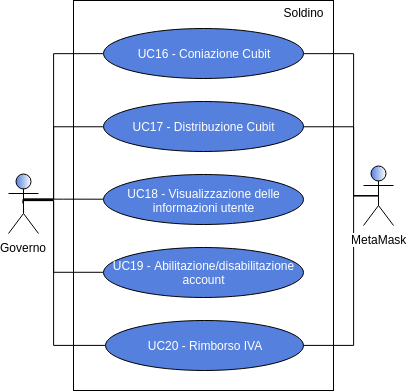
\includegraphics[width=7cm]{res/images/UC-Governo.png}
	\centering
	\caption{Schema generale: casi d'uso governativi}
\end{figure}
\subsubsection{UC16 - Coniazione Cubit}
\begin{itemize}
	\item \textbf{Attori Primari}: governo;
	\item \textbf{Attori Secondari}: MetaMask\glo;
	\item \textbf{Descrizione}: viene coniata una quantità definita di Cubit\glo;
	
	\item \textbf{Scenario principale}: il governo ritiene necessario coniare ulteriori Cubit rispetto a quelli attualmente presenti sul mercato. Per fare ciò deve accedere alla pagina dedicata in cui, attraverso un form dovrà:
	 \begin{enumerate}[label=\alph*.]
		\item inserire la quantità $x$ di Cubit da coniare;
		\item confermare tale operazione attraverso l'utilizzo di MetaMask\glo.
	\end{enumerate}
	\item \textbf{Precondizione}: sia $x$ l'ammontare di Cubit che il governo 
	vuole coniare e $n$ l'ammontare di Cubit attualmente in circolo. L'utente 
	governativo ha acceduto alla pagina per la coniazione ed ha compilato e 
	confermato il form;
	\item \textbf{Postcondizione}: i Cubit in circolo sono $x+n$.
\end{itemize}
\subsubsection{UC17 - Distribuzione Cubit}
%non capisco perchè la figura è prima del titolo sul PDF
\begin{figure}[h]
	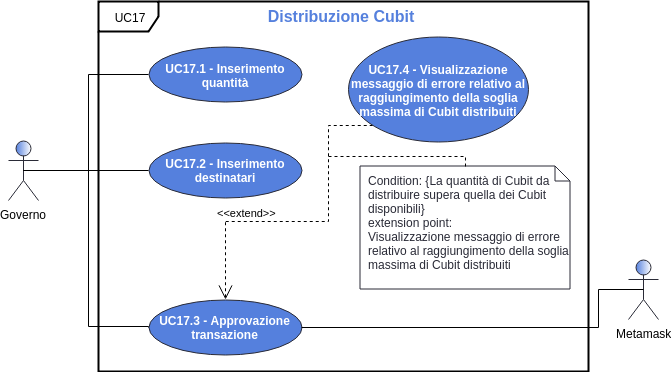
\includegraphics[width=13.5cm]{res/images/UC17.png} %da adattare in larghezza
	\centering
	\caption{UC17 - Distribuzione Cubit}
	
\end{figure}
\begin{itemize}
	\item \textbf{Attori Primari}: governo;
	\item \textbf{Attori Secondari}: MetaMask\glo;
	\item \textbf{Descrizione}: il governo trasferisce una somma di Cubit\glosp sull'account di uno o più  utenti, che siano essi cittadini o aziende;
	\item \textbf{Scenario principale}: il governo deve:
	 \begin{enumerate}[label=\alph*.]
		\item determinare l'ammontare di Cubit pro capite da trasferire [UC17.1];
		\item  selezionare la lista dei destinatari del trasferimento dalla lista degli utenti [UC17.2];
		\item confermare l'operazione [UC17.3].
	\end{enumerate}

	\item \textbf{Precondizione}: il governo accede alla pagina contenente il form per la distribuzione di Cubit agli utenti e compila il suddetto form;
	\item \textbf{Postcondizione}: tali utenti ricevono i Cubit da parte del governo.
\end{itemize}
\subsubsection{UC17.1 - Inserimento quantità}
\begin{itemize}
	\item \textbf{Attori Primari}: governo;
	\item \textbf{Descrizione}: il governo inserisce nell'apposito campo del form la quantità di Cubit\glosp da distribuire, ritenendo la quantità inserita come quantità da inviare ad ogni singolo utente;
	\item \textbf{Scenario principale}: il governo inserisce l'ammontare $x$ di 
	Cubit da inviare;
	\item \textbf{Precondizione}: il governo si trova alla pagina contenente il form per la distribuzione di Cubit agli utenti;
	\item \textbf{Postcondizione}: il campo relativo all'ammontare di Cubit da 
	distribuire pro capite è stato compilato. 
\end{itemize}
\subsubsection{UC17.2 - Inserimento destinatari}
\begin{itemize}
	\item \textbf{Attori Primari}: governo;
	\item \textbf{Descrizione}: il governo inserisce nell'apposito form la lista dei destinatari della quantità di Cubit\glosp precedentemente inserita;
	\item \textbf{Scenario principale}: il governo:
	\begin{enumerate}[label=\alph*.]
		\item visualizza delle liste contenenti i cittadini e le aziende registrate al sito, che sono accompagnati da una checkbox;
		\item l'utente può usare una barra di ricerca per individuare dei particolari utenti;
		\item l'utente governativo spunta le caselle relative agli utenti ai quali intende trasferire la quantità di Cubit precedentemente definita.
	\end{enumerate}
	\item \textbf{Precondizione}: il governo si trova nella pagina atta alla distribuzione dei Cubit e ha selezionato la quantità di Cubit da distribuire;
	\item \textbf{Postcondizione}: il governo ha selezionato uno o più destinatari dalle liste degli utenti e può procedere con l'approvazione della transazione.
\end{itemize}
\subsubsection{UC17.3 - Approvazione transazione}
\begin{itemize}
	\item \textbf{Attori Primari}: governo;
	\item \textbf{Attori Secondari}: MetaMask\glo;
	\item \textbf{Descrizione}: il governo decide se approvare o rifiutare la transazione;
	\item \textbf{Scenario principale}: il governo ha specificato la somma 
	$x$ di Cubit\glosp da distribuire ad ognuno degli $y$ destinatari;
	\item \textbf{Estensioni}:
	\begin{itemize}
		\item \textbf{UC17.4}: verrà mostrato un messaggio di errore nel caso 
		l'ammontare totale $x\cdot y$ superi la quantità di Cubit disponibili 
		alla distribuzione.
	\end{itemize}
	\item \textbf{Precondizione}: è necessario aver selezionato una lista di destinatari ed una quantità da distribuire ad ogni singolo utente;
	\item \textbf{Postcondizione}: ogni utente riceverà nel proprio wallet\glosp la quantità di Cubit trasferita dal governo.
\end{itemize}
\subsubsection{UC17.4 - Visualizzazione messaggio di errore relativo al raggiungimento della soglia massima di Cubit distribuiti}
\begin{itemize}
	\item \textbf{Attori Primari}: governo;
	\item \textbf{Descrizione}: il governo riceve un messaggio di errore relativo al fatto che ha selezionato una quantità di Cubit\glosp superiore a quella disponibile alla distribuzione;
	\item \textbf{Scenario principale}: il governo clicca sull'apposito pulsante per confermare la transazione di distribuzione, ma non ha sufficienti fondi per completare tale operazione;
	\item \textbf{Precondizione}: il governo deve aver inserito una quantità di Cubit superiore a quella disponibile e cerca di effettuare la transazione;
	\item \textbf{Postcondizione}: viene visualizzato un messaggio d'errore per informare l'utente del fatto che attualmente non dispone dei fondi necessari per effettuare l'operazione di distribuzione.
	
\end{itemize} 
